\documentclass{article}
\usepackage{graphicx} % Required for inserting images
\usepackage{amsmath}
\usepackage{tikz}

\title{Worksheet \#4}
\author{Rosa Orellana}
\date{August 6, 2026}

\begin{document}

\maketitle
\begin{enumerate}
\item Explain why the chromatic symmetric function is symmetric. 
%\item Explain why if the graph is disconnected and contains two 
%components, then its chromatic symmetric function is the product of the chromatic symmetric function of the two components of the graph. 
\item Let $G$ be a graph and $e$ an edge in $G$. In graph theory the chromatic polynomial is computed using the deletion-contraction recurrence: 
\[\chi_G(n) = \chi_{G-e}(n) -\chi_{G/e}(n), \] where $G-e$ is the graph with the edge $e$ removed and with the same vertices as $G$, and $G/e$ is the graph with the edge $e$ contracted to single vertex. If multiple edges result, you replace them with a single edge. 
Use this recurrence to compute the chromatic polynomial of the cycle graph with four vertices (the image is in Problem \#3).

Recall that the chromatic polynomial of a tree, $T$,  with $k$ vertices is $\chi_T(n) = n(n-1)^{k-1}$

\item Take the cycle graph with four vertices and choose one edge. 
\begin{center}
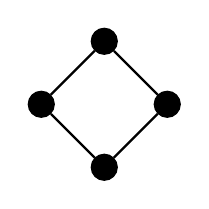
\begin{tikzpicture}[scale=0.4, auto, 
    vertex/.style={circle, draw, fill=black, minimum size=.5mm}]

    % Define vertices with coordinates
    \node[vertex] (v1) at (0,2) {};
    \node[vertex] (v2) at (2,0) {};
    \node[vertex] (v3) at (0,-2) {};
    \node[vertex] (v4) at (-2,0) {};
    % Draw edges connecting the vertices in a cycle
    \draw[thick] (v1) -- (v2) -- (v3) -- (v4) -- (v1);
\end{tikzpicture}
\end{center}
\begin{enumerate}
    \item What graph do you get when you delete this edge? Compute the chromatic symmetric function for the graph that you get in the power sum basis. 
    \item What graph do you get when you contract this edge? Compute the chromatic symmetric function for the graph that you get in the power sum basis. 
    \item Using this example, explain why the chromatic symmetric function does not satisfy the deletion-contraction recurrence. 
\end{enumerate}

\item A tree with $k$ vertices can be defined as a connected graph with $k-1$ edges. 
\begin{enumerate}
\item In our lecture we said that all trees have chromatic polynomial equal to $n(n-1)^{k-1}$.  Use the binomial theorem,
\[
(a+b)^m = \sum_{i=0}^m \binom{m}{i} a^ib^{m-i},
\]
to expand this polynomial. 
\item What is the coefficient of $n^{k-1}$? 
\item Use induction and the deletion-contraction recurrence to show that the coefficient of $n^{k-1}$ in $\chi_G(n)$ is equal to the negative of the number of edges in $G$. 
\item Suppose that $G$ is a connected graph with $k$ vertices and $\chi_G(n) = n(n-1)^{k-1}$, explain why $G$ must be a tree. 
\end{enumerate}

\item Compute the chromatic symmetric function of the following graphs in the monomial basis. 

\begin{center}
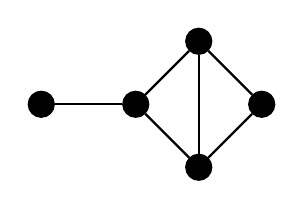
\begin{tikzpicture}[scale=0.4, auto, 
    vertex/.style={circle, draw, fill=black, minimum size=.5mm}]

    % Define vertices with coordinates
    \node[vertex] (v1) at (0,2) {};
    \node[vertex] (v2) at (2,0) {};
    \node[vertex] (v3) at (0,-2) {};
    \node[vertex] (v4) at (-2,0) {};
    \node[vertex] (v5) at (-5,0) {};
    % Draw edges connecting the vertices in a cycle
    \draw[thick] (v1) -- (v2) -- (v3) -- (v4) -- (v1);
    \draw[thick]  (v1) -- (v3);
    \draw[thick]  (v4) -- (v5);
\end{tikzpicture}
\hskip 1in
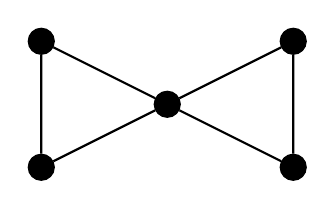
\begin{tikzpicture}[scale=0.4, auto, 
    vertex/.style={circle, draw, fill=black, minimum size=.5mm}]

    % Define vertices with coordinates
    \node[vertex] (v1) at (-2,-2) {};
    \node[vertex] (v2) at (-2,2) {};
    \node[vertex] (v3) at (6,2) {};
    \node[vertex] (v4) at (6, -2) {};
    \node[vertex] (v5) at (2,0) {};
    % Draw edges connecting the vertices in a cycle
    \draw[thick] (v1) -- (v5) -- (v2) -- (v1);
    \draw[thick] (v4)--(v3) -- (v5) -- (v4);
    
\end{tikzpicture}
\end{center}
\item Given $X_G$ for some graph $G$ in the power basis, how can you tell whether $G$ is connected or not from the coefficients?  

\item Show that if $G$ and $H$ satisfy $X_G = X_H$, then $G$ and $H$ must have the same number of edges. 

\item Compute the chromatic symmetric function of the complete graph for $n\leq 5$ vertices in the elementary basis.   Conjecture a formula for the chromatic symmetric function of the complete graph. 

\item Let $G$ be a graph with a leaf edge $e$, 
\begin{enumerate}
    \item Describe the graph that you get when you delete $e$. 
    \item Describe the graph that you get when you do a dot-contraction to $e$. 
    \item How are the graphs that you got in (a) and in (b) related?
    \item What graph do you get when you leaf-contract the edge $e$?
    \item How does this justify that we only apply deletion-near-contraction to internal edges? 
\end{enumerate}

 
\item Use the deletion-near-contraction relation to find the chromatic symmetric function of all trees with 5 vertices in the star basis. 

\item  Compute the chromatic symmetric function of the following two graphs in the star basis. 

\begin{center}
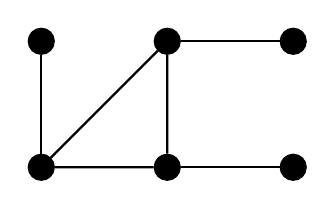
\begin{tikzpicture}[scale=0.4, auto, 
    vertex/.style={circle, draw, fill=black, minimum size=.5mm}]

    % Define vertices with coordinates
    \node[vertex] (v1) at (-2,-2) {};
    \node[vertex] (v2) at (2,-2) {};
    \node[vertex] (v3) at (2,2) {};
    \node[vertex] (v4) at (-2,2) {};
    \node[vertex] (v5) at (6,2) {};
    \node[vertex] (v6) at (6, -2) {};
    % Draw edges connecting the vertices in a cycle
    \draw[thick] (v1) -- (v3)-- (v2) -- (v1); 
    \draw[thick] (v3) -- (v5);
    \draw[thick]  (v1) -- (v4);
    \draw[thick]  (v2) -- (v6);
\end{tikzpicture}
\hskip 1in 
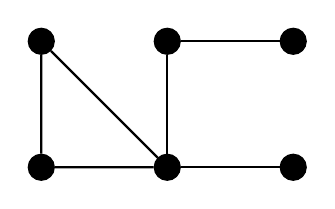
\begin{tikzpicture}[scale=0.4, auto, 
    vertex/.style={circle, draw, fill=black, minimum size=.5mm}]

    % Define vertices with coordinates
    \node[vertex] (v1) at (-2,-2) {};
    \node[vertex] (v2) at (2,-2) {};
    \node[vertex] (v3) at (2,2) {};
    \node[vertex] (v4) at (-2,2) {};
    \node[vertex] (v5) at (6,2) {};
    \node[vertex] (v6) at (6, -2) {};
    % Draw edges connecting the vertices in a cycle
    \draw[thick] (v1) -- (v4)-- (v2) -- (v1); 
    \draw[thick] (v3) -- (v5);
    \draw[thick]  (v2) -- (v3);
    \draw[thick]  (v2) -- (v6);
\end{tikzpicture}
\end{center}







\end{enumerate}
\newpage
\section*{Español}
\begin{enumerate}
\item Explique por qué la función simétrica cromática es una función simétrica.

\item Sea $G$ un grafo y $e$ una arista en $G$. En teoría de grafos, el polinomio cromático se calcula usando la relación de eliminación-contracción:
\[\chi_G(n) = \chi_{G-e}(n) -\chi_{G/e}(n), \] donde $G-e$ es el grafo con la arista $e$ eliminada y con los mismos vértices que $G$, y $G/e$ es el grafo que se obtiene al contraer la arista $e$ a un solo vértice. Si resultan múltiples aristas, reemplácelas por una sola arista.
Usando esta relación, calcule el polinomio cromático del grafo cíclico de cuatro vértices (la imagen del Problema \#3).

Recuerde que el polinomio cromático de un árbol $T$ con $k$ vértices es $\chi_T(n) = n(n-1)^{k-1}$.

\item Tome el grafo cíclico con cuatro vértices y elija una arista.
\begin{center}
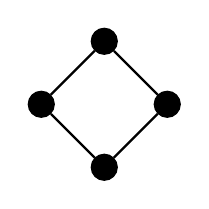
\begin{tikzpicture}[scale=0.4, auto, 
    vertex/.style={circle, draw, fill=black, minimum size=.5mm}]

    % Define vertices with coordinates
    \node[vertex] (v1) at (0,2) {};
    \node[vertex] (v2) at (2,0) {};
    \node[vertex] (v3) at (0,-2) {};
    \node[vertex] (v4) at (-2,0) {};
    % Draw edges connecting the vertices in a cycle
    \draw[thick] (v1) -- (v2) -- (v3) -- (v4) -- (v1);
\end{tikzpicture}
\end{center}
\begin{enumerate}
    \item ¿Qué grafo obtiene al eliminar esta arista? Calcule la función simétrica cromática del grafo obtenido en la base de sumas de potencias.
    \item ¿Qué grafo obtiene al contraer esta arista? Calcule la función simétrica cromática del grafo obtenido en la base de sumas de potencias.
    \item Usando este ejemplo, explique por qué la función simétrica cromática no satisface la relación de eliminación-contracción.
\end{enumerate}

\item Un árbol con $k$ vértices puede definirse como un grafo conexo con $k-1$ aristas.
\begin{enumerate}
\item En clase dijimos que todos los árboles tienen polinomio cromático igual a $n(n-1)^{k-1}$. Use el teorema del binomio,
\[
(a+b)^m = \sum_{i=0}^m \binom{m}{i} a^ib^{m-i},
\]
para expandir este polinomio.
\item ¿Cuál es el coeficiente de $n^{k-1}$?
\item Use inducción y la relación de eliminación-contracción para demostrar que el coeficiente de $n^{k-1}$ en $\chi_G(n)$ es igual al negativo del número de aristas de $G$.
\item Suponga que $G$ es un grafo conexo con $k$ vértices y $\chi_G(n) = n(n-1)^{k-1}$; explique por qué $G$ debe ser un árbol.
\end{enumerate}

\item Calcule la función simétrica cromática de los siguientes grafos en la base monomial.

\begin{center}
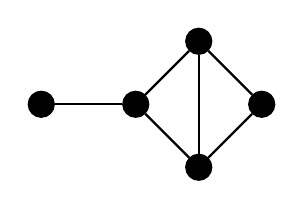
\begin{tikzpicture}[scale=0.4, auto, 
    vertex/.style={circle, draw, fill=black, minimum size=.5mm}]

    % Define vertices with coordinates
    \node[vertex] (v1) at (0,2) {};
    \node[vertex] (v2) at (2,0) {};
    \node[vertex] (v3) at (0,-2) {};
    \node[vertex] (v4) at (-2,0) {};
    \node[vertex] (v5) at (-5,0) {};
    % Draw edges connecting the vertices in a cycle
    \draw[thick] (v1) -- (v2) -- (v3) -- (v4) -- (v1);
    \draw[thick]  (v1) -- (v3);
    \draw[thick]  (v4) -- (v5);
\end{tikzpicture}
\hskip 1in
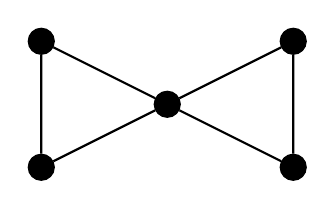
\begin{tikzpicture}[scale=0.4, auto, 
    vertex/.style={circle, draw, fill=black, minimum size=.5mm}]

    % Define vertices with coordinates
    \node[vertex] (v1) at (-2,-2) {};
    \node[vertex] (v2) at (-2,2) {};
    \node[vertex] (v3) at (6,2) {};
    \node[vertex] (v4) at (6, -2) {};
    \node[vertex] (v5) at (2,0) {};
    % Draw edges connecting the vertices in a cycle
    \draw[thick] (v1) -- (v5) -- (v2) -- (v1);
    \draw[thick] (v4)--(v3) -- (v5) -- (v4);
    
\end{tikzpicture}
\end{center}

\item Dado $X_G$ para algún grafo $G$ en la base de sumas de potencias, ¿cómo puede determinar a partir de los coeficientes si $G$ es conexo o no?

\item Demuestre que si $G$ y $H$ satisfacen $X_G = X_H$, entonces $G$ y $H$ deben tener el mismo número de aristas.

\item Calcule la función simétrica cromática del grafo completo para $n\leq 5$ vértices en la base elemental. Conjeture una fórmula para la función simétrica cromática del grafo completo.

\item Sea $G$ un grafo con una arista hoja $e$:
\begin{enumerate}
    \item Describa el grafo que obtiene al eliminar $e$.
    \item Describa el grafo que obtiene al aplicar una contracción-punto (\emph{dot-contraction}) a $e$.
    \item ¿Cómo se relacionan los grafos que obtuvo en (a) y (b)?
    \item ¿Qué grafo obtiene al aplicar una contracción-hoja (\emph{leaf-contraction}) a la arista $e$?
    \item ¿Cómo justifica esto que solo apliquemos la eliminación-\allowbreak cerca-de-\allowbreak contracción (\emph{deletion-near-contraction}) a aristas internas?
\end{enumerate}

\item Use la relación de eliminación-cerca-de-contracción, en inglés \emph{deletion-near-contraction}, para encontrar la función simétrica cromática de todos los árboles con 5 vértices en la base de estrellas (\emph{star basis}).

\item Calcule la función simétrica cromática de los siguientes dos grafos en la base de estrellas.

\begin{center}
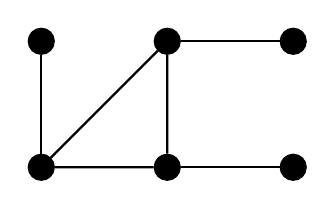
\begin{tikzpicture}[scale=0.4, auto, 
    vertex/.style={circle, draw, fill=black, minimum size=.5mm}]

    % Define vertices with coordinates
    \node[vertex] (v1) at (-2,-2) {};
    \node[vertex] (v2) at (2,-2) {};
    \node[vertex] (v3) at (2,2) {};
    \node[vertex] (v4) at (-2,2) {};
    \node[vertex] (v5) at (6,2) {};
    \node[vertex] (v6) at (6, -2) {};
    % Draw edges connecting the vertices in a cycle
    \draw[thick] (v1) -- (v3)-- (v2) -- (v1); 
    \draw[thick] (v3) -- (v5);
    \draw[thick]  (v1) -- (v4);
    \draw[thick]  (v2) -- (v6);
\end{tikzpicture}
\hskip 1in 
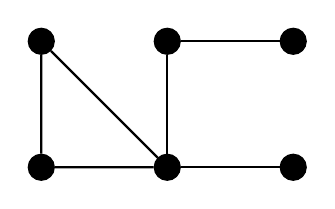
\begin{tikzpicture}[scale=0.4, auto, 
    vertex/.style={circle, draw, fill=black, minimum size=.5mm}]

    % Define vertices with coordinates
    \node[vertex] (v1) at (-2,-2) {};
    \node[vertex] (v2) at (2,-2) {};
    \node[vertex] (v3) at (2,2) {};
    \node[vertex] (v4) at (-2,2) {};
    \node[vertex] (v5) at (6,2) {};
    \node[vertex] (v6) at (6, -2) {};
    % Draw edges connecting the vertices in a cycle
    \draw[thick] (v1) -- (v4)-- (v2) -- (v1); 
    \draw[thick] (v3) -- (v5);
    \draw[thick]  (v2) -- (v3);
    \draw[thick]  (v2) -- (v6);
\end{tikzpicture}
\end{center}

\end{enumerate}

\end{document}
